\subsection{Use Cases}
\label{sec:verso_use_cases}

Throughout the timespan of the present thesis, the VRS and, specifically, the VERSO software infrastructure
has been used in a wide variety of settings and for many purposes.
In this section a few such use-cases will be highlighted.

\subsubsection{Test Benches}
\label{sec:verso_test_bench}

For the majority of studies of the frontend electronics, namely the frontend boards
and the VMM ASIC, detectors are not needed.
For this reason, one of the primary uses of the VRS and VERSO DAQ and calibration software
is in testbenches in electronics labs.
A typical setup is shown in Figure~\ref{fig:vrs_testbench}.
The use of VRS in the testbench allows for quick and direct inspection
of the frontend electronics via an oscilloscope.
In such a setup, the response of the frontend electronics to communications sent
from VERSO to the FGPA (or the FPGA to the VMM), and vice versa, can immediately be seen
by visual means.
Calibration and off-detector performance of the frontend electronics and VMM can also be studied
in the `clean' scenarios provided by the testbench setup.
Use in labs and testbenches has allowed for the VRS software and firmware to be fully validated and for
the validation of the NSW frontend boards as they have evolved.

\begin{figure}[!htb]
    \begin{center}
        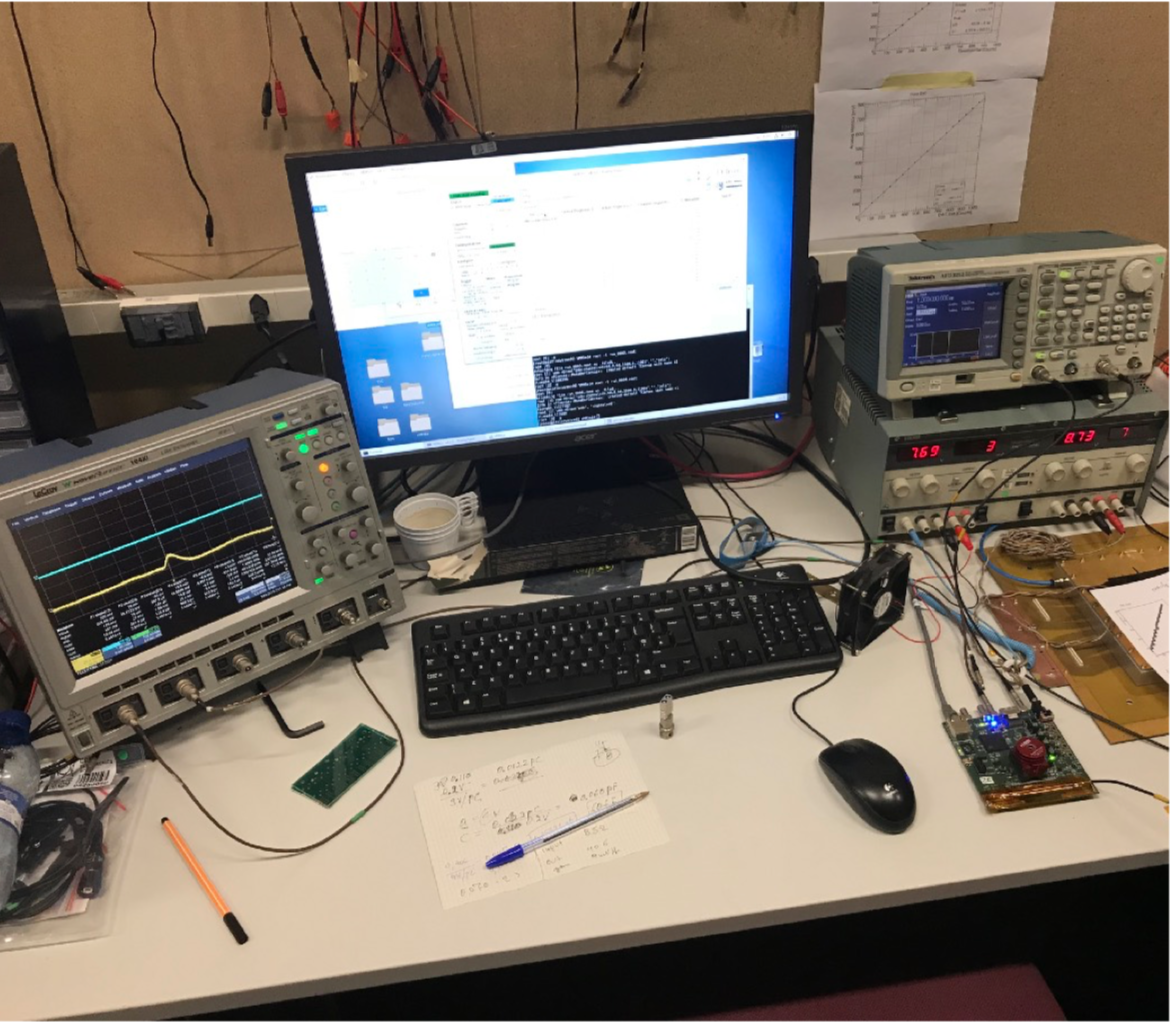
\includegraphics[width=0.49\textwidth]{figures/nsw/use_cases/verso_use_case_vs_socket}
        \raisebox{0.28cm}{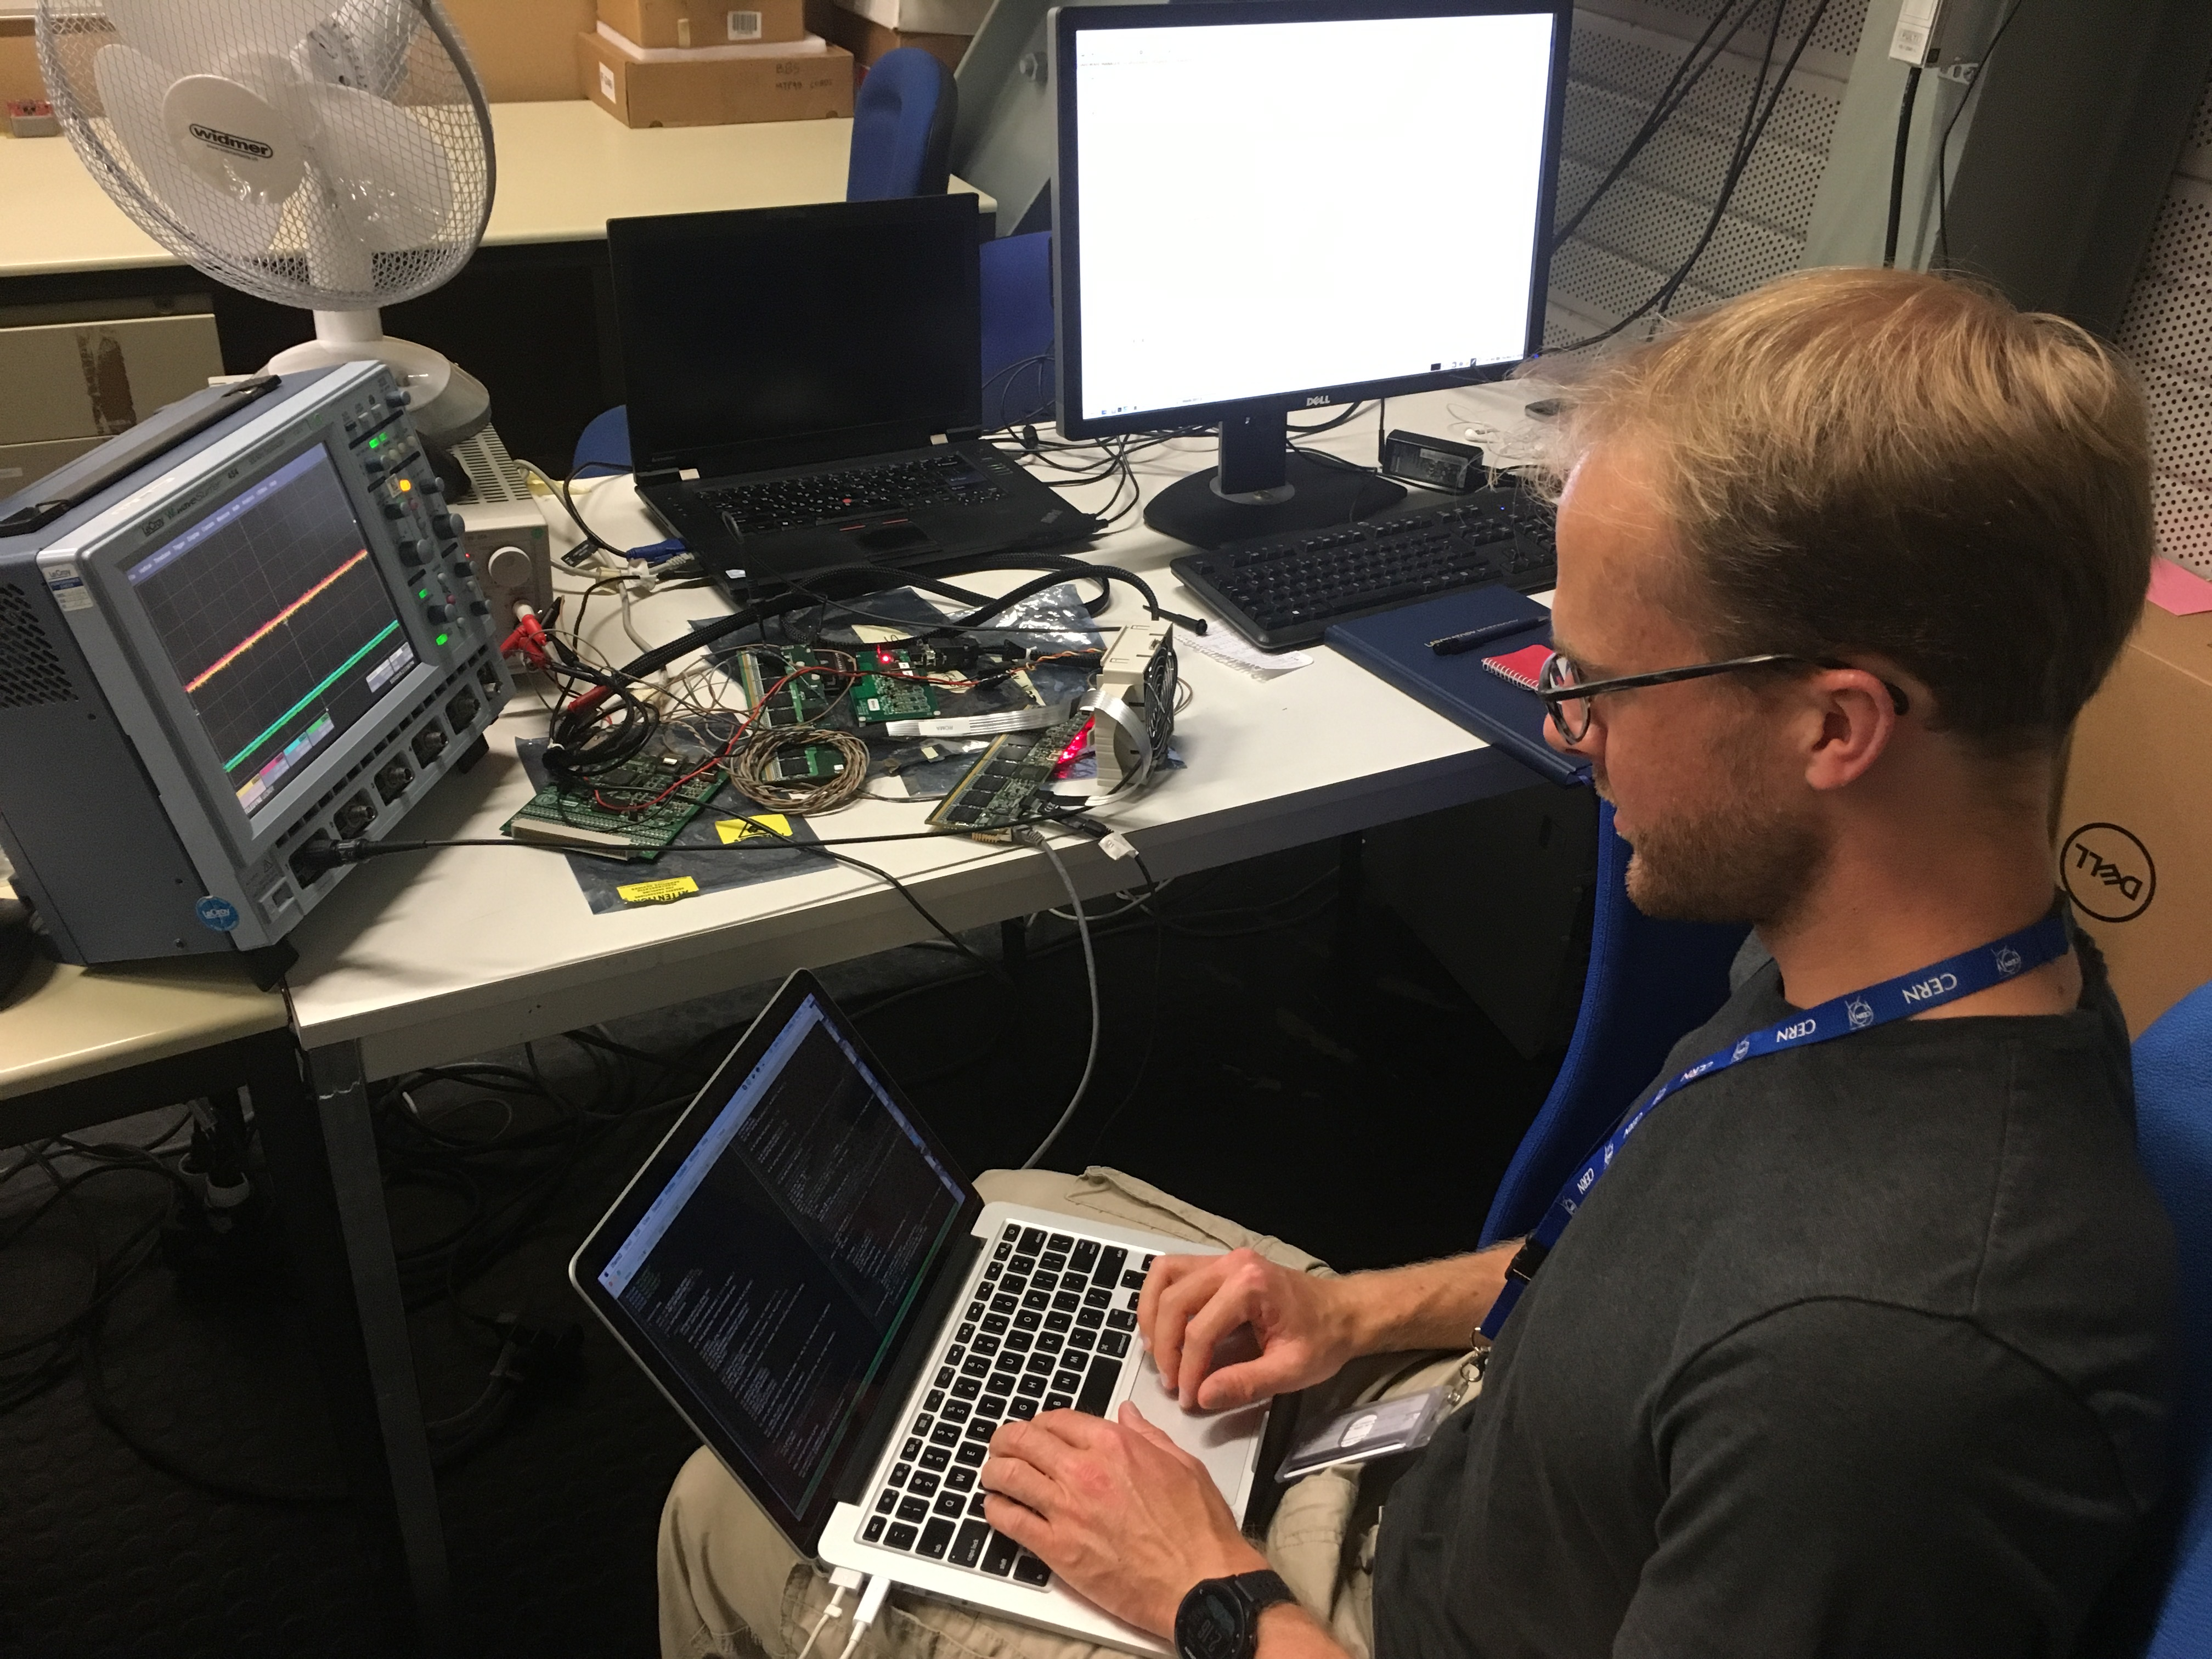
\includegraphics[width=0.49\textwidth]{figures/nsw/use_cases/vrs_dantrim}}
        \caption{
            \textbf{\textit{Left}}: A typical VRS testbench setup.
                The frontend board housing the VMM is seen in the picture on the lower right (GPVMM-type frontend board).
                An oscilloscope is available for probing the frontend board and VMM outputs visually.
                The frontend board is connected to the shown PC via a direct Ethernet connection.
                A function generator producing input signals is at the right, being used to test the injection
                of signals independently from the VMM channel test charge capacitors.
            \textbf{\textit{Right}}: Another example of a typical testbench setup, with the present
                author hard at work.
                In this case, VERSO is hosted on a single laptop with a direct Ethernet connection to the frontend board.
                The frontend board in this case is an MMFE8-type frontend board.
                In the case shown, the VRS firmware on the frontend board is being debugged.
                The PC at the upper right, connected to the frontend board via a mini-SAS connection, is responsible for writing and uploading the firmware to the
                on-board FPGA.
        }
        \label{fig:vrs_testbench}
    \end{center}
\end{figure}

\subsubsection{Cosmic Stand}
\label{sec:verso_cosmic}

The VRS system has also been used to collect cosmic muon data from instrumented detectors, on cosmic stands
located in NSW labs at CERN and elsewhere.
One such example is shown in Figure~\ref{fig:mm_quad_elx}, showing the large-scale MM chambers
in the cosmic stand located at the RD51 lab at CERN.
Another, more recent (at the time of writing) example is that of the final MM detector integration
site whereat the final NSW MM chambers are being assembled.
As the final DAQ system that will be used once the NSW is installed in ATLAS is not yet fully ready,
at the time of writing, the VRS system was used to configure and readout the frontend electronics
interfaced to the final full-scale MM double-wedges.
For the final integration, noise tests of the electronics on the final MM detectors that will be
installed in ATLAS are needed in order to verify the base performance of the large-scale detectors.
The double-wedge MM detectors are additionally placed onto a cosmic-ray stand and initial data was able to be
collected with the VRS and VERSO DAQ software.
The VRS system, in this case, helped allow for the final NSW MM integration procedures to be put into place
while the full-scale DAQ infrastructure to be used once the NSW is installed in ATLAS was made available.

\begin{figure}[!htb]
    \begin{center}
        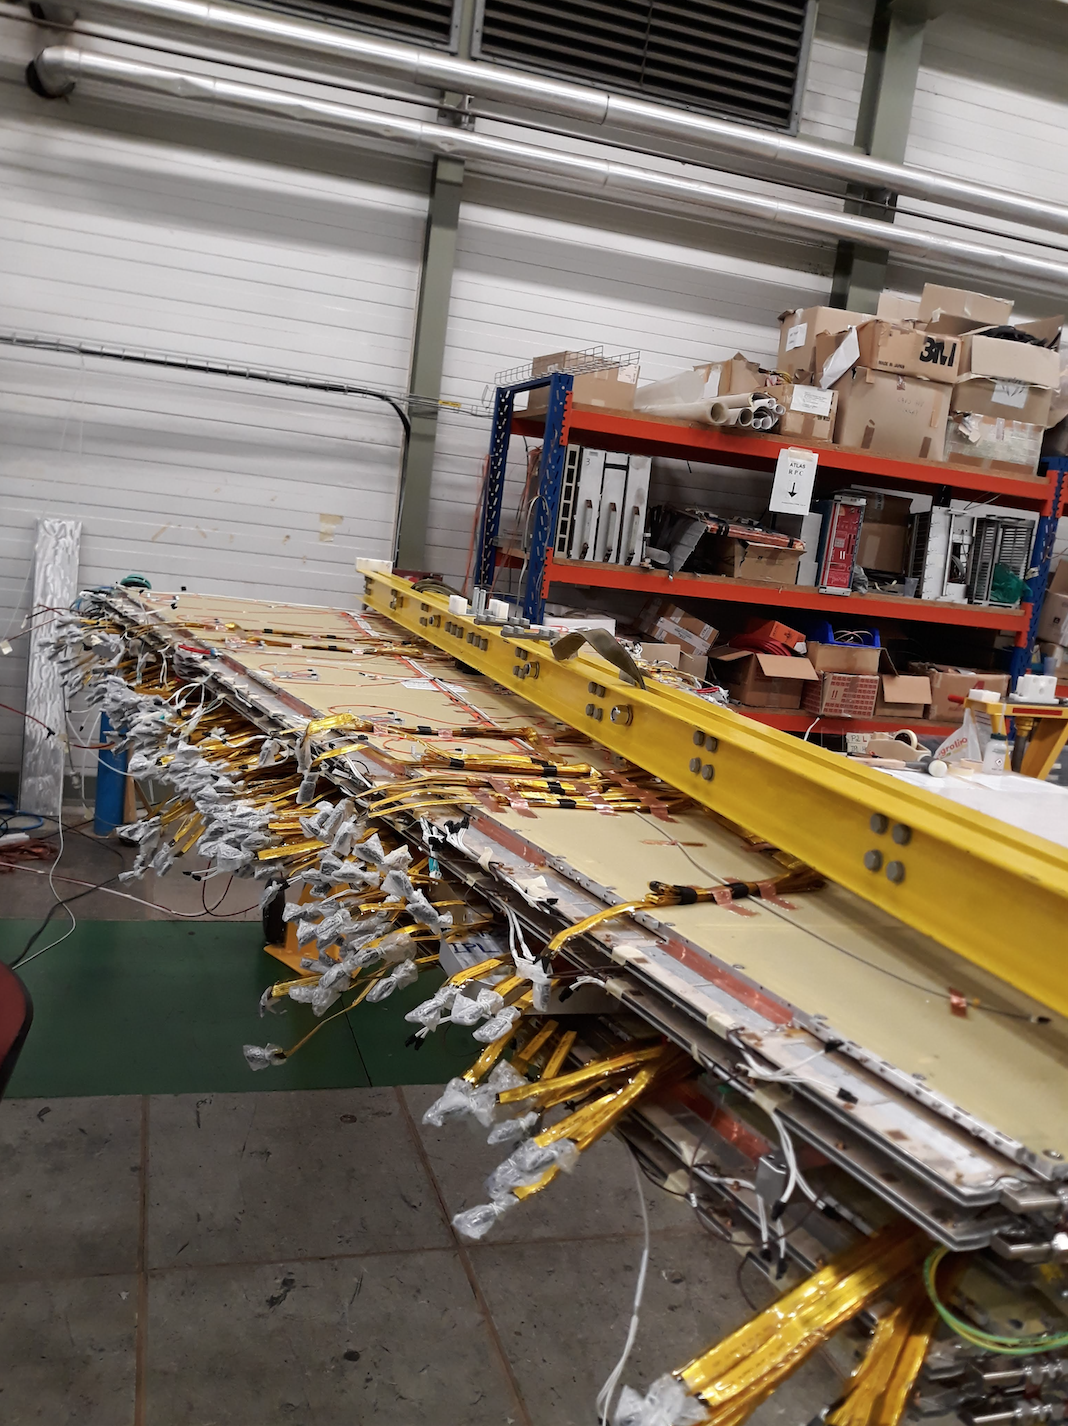
\includegraphics[width=0.48\textwidth]{figures/nsw/use_cases/mm_bb5}
        \raisebox{2.5cm}{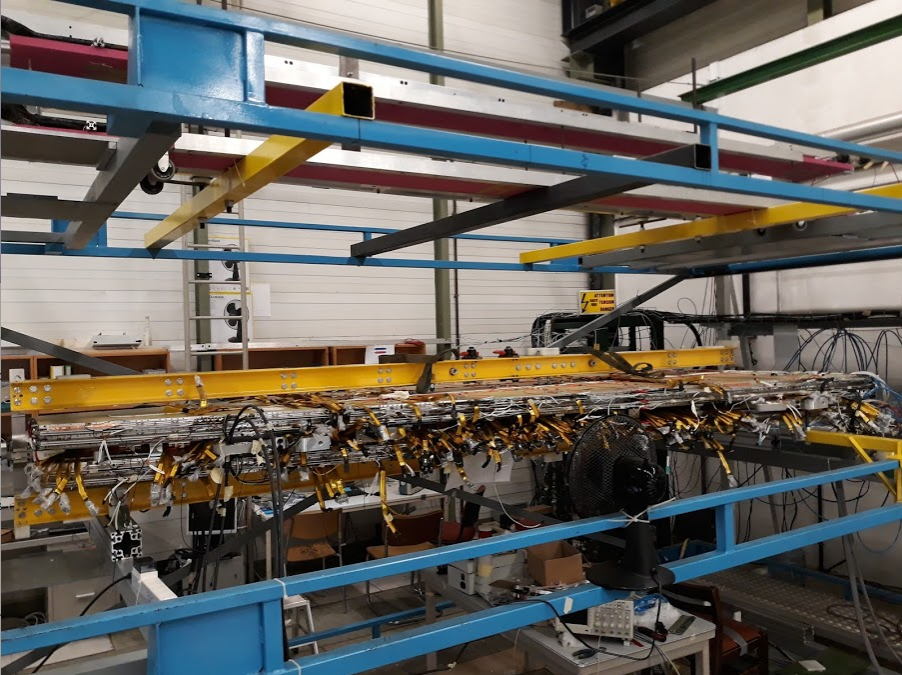
\includegraphics[width=0.48\textwidth]{figures/nsw/use_cases/mm_bb5_cosmic}}
        \caption{
            \textbf{\textit{Left}}: Assembled NSW MM sector (double-wedge) at the MM integration
                site at CERN.
            \textbf{\textit{Right}}: MM sector on the cosmic-ray test-stand at the MM integration site
                at CERN. The detector is instrumented with MMFE8 frontend boards with Ethernet readout
                achieved via the VRS and VERSO DAQ software, hosted on the PC located just behind the cosmic
                stand.
        }
        \label{fig:mm_bb5}
    \end{center}
\end{figure}


\subsubsection{Frontend Board Validation}
\label{sec:verso_noise}

The design of the frontend board to be used in the NSW was being finalised throughout the timespan
of this thesis.
In order to validate that the frontend board met the standards required for operation in the NSW, specifically
that it did not introduce too much electronics noise as a result of its design,
the VRS system and VERSO software were required.
The prototype boards, then, for the NSW are all outfitted with an FPGA and Ethernet connector as in Figure~\ref{fig:frontend_boards}
so that they can be interfaced with the VRS readout system.
The main goals of the frontend board validation are to ensure proper routing between the VMM
ASIC and the rest of the frontend board elements which can be tested by verifying the VMM's response
to specific configuration commands.
Noise tests are also performed by measuring the frontend board noise as described in Section~\ref{sec:calib_baselines}.
Such an example of a noise tests using prototype MMFE8s while interfaced to full-scale MM detector chambers
is shown in Figure~\ref{fig:mm_quad_elx}.
Performing such tests allow, also, to verify that the physical connections between the frontend electronics and detectors, such as the ZEBRA connectors in the
case of the MM detectors,
are without fault. Any such fault would appear as a faulty set of channels only when the electronics
are interfaced to the detector, for example.

\subsubsection{Testbeams}
\label{sec:verso_testbeam}

\begin{figure}[!htb]
    \begin{center}
        \raisebox{1.8cm}{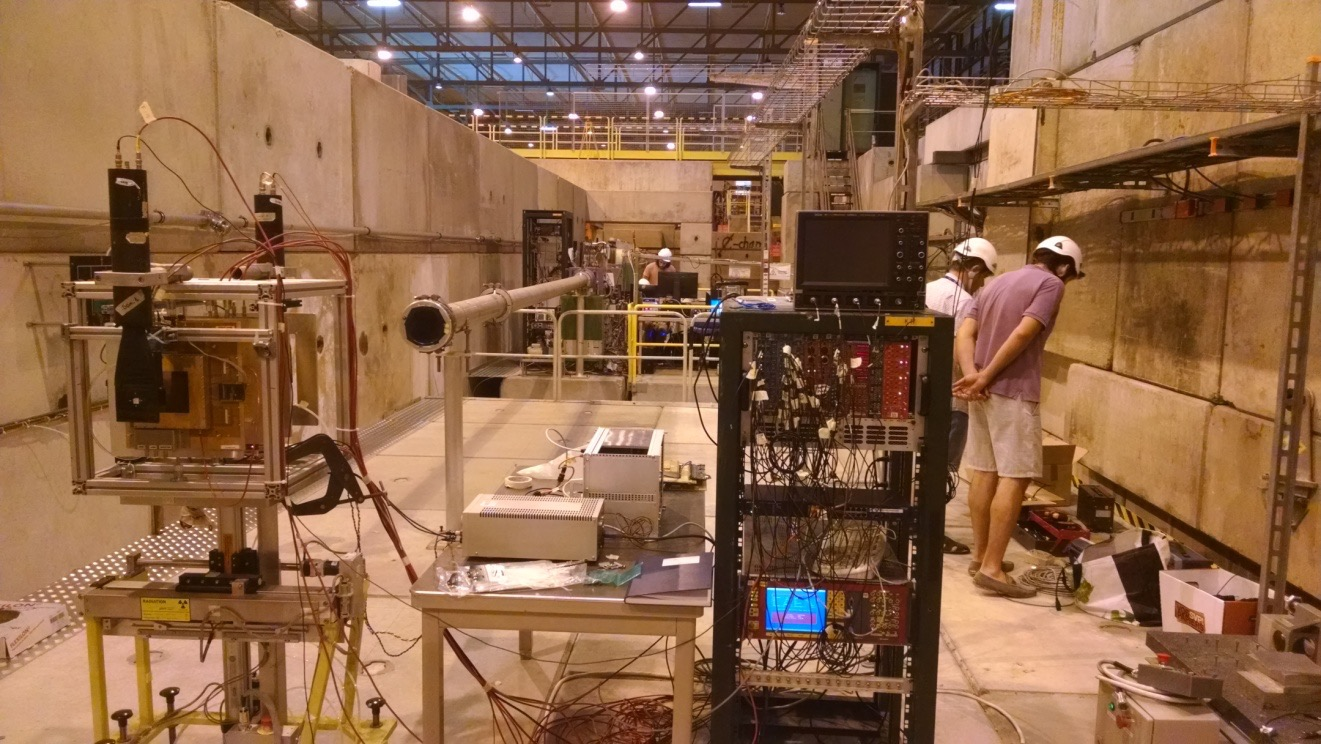
\includegraphics[width=0.58\textwidth]{figures/nsw/use_cases/vrs_testbeam}}
        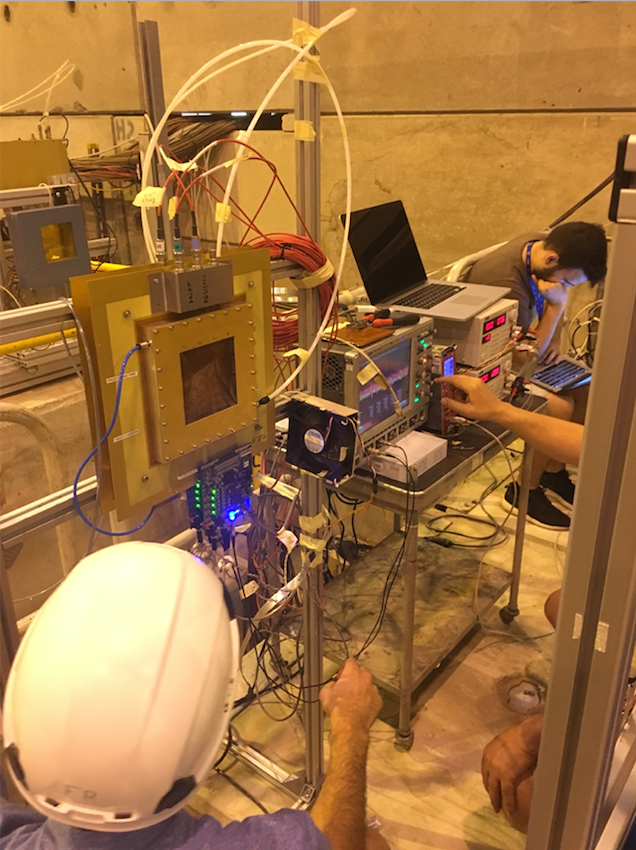
\includegraphics[width=0.4\textwidth]{figures/nsw/use_cases/verso_testbeam2}
        \caption{
            \textbf{\textit{Left}}: Typical testbeam setup at the CERN North Area, located at the Prevessin Site at CERN.
                The small prototype MM chambers are housed in the aluminum frame on the left with scintillator
                trigger paddles on either side.
                The beam tunnel can be seen extending into the distance.
                The trigger and high voltage systems are seen on the rack in the middle of the picture.
                The DAQ PC is housed in a control room (not shown) some 10-15\,m outside of the beam area.
            \textbf{\textit{Right}}: A close up of a small prototype MM chamber at a test beam. The
                GPVMM-type frontend board is interfaced at the bottom. Here it can be seen that there
                are two MM chambers back-to-back, each with a frontend board attached at their bottom.
                The cables providing high voltage (in red) and gas (white) to the MM chambers are seen, as well.
        }
        \label{fig:vrs_testbeam}
    \end{center}
\end{figure}

From 2016 until the present time of writing, the VRS system and VERSO DAQ software have been used as the main DAQ infrastructure
for test beam campaigns at CERN.
The testbeam area at CERN is located at the CERN Prevessin site, in the North Area.
Proton beams from the SPS are made to collide with a fixed target upstream of the detectors and
the collision products are sent through several beamlines in the North Area along which
detectors can be placed.
The beams from the SPS are extracted roughly every 40\,seconds and particles are sent down the beamlines towards
the detectors for roughly 5\,second `spills'.
In such cases, the particle rates observed at the detectors are on the order of several 100\,kHz.
The main purpose of these testbeam campaigns was to verify the performance of both the VMM ASIC and prototype NSW frontend
boards in high-rate environments.
The VRS system and VERSO DAQ software have succeeded in recording data at 100\% efficiency at these
rates, allowing for high volumes of data to be collected and used in NSW detector performance and electronics studies.
For such data, used to validate the frontend electronics and tracking performance of NSW-type detectors in realistic data-taking environments,
the calibration routines described in Section~\ref{sec:calib_alg}, and implemented within the VERSO software infrastructure, are of the utmost importance.

\subsubsection{VMM Production Validation}
\label{sec:verso_vmm_prod}

Throughout the work presented in this thesis, the VMM ASIC has gone through 3 versions.
In order to validate that a given VMM production is adequate --- meaning that there is no systematic
fault in the ASIC production, for example --- large scale tests of all ASICs produced in manufacturing test runs 
are required.
In many cases, the automated calibration routines supported by VERSO were required to perform these production
tests.
In one such case, the manufacturing process of the silicon wafers used to produce the VMM was changed
and in order to verify that the resulting changes observed on the VMM performance were due to this
change, a direct study of the VMM characteristics prior to the changed process being applied
to the silicon was needed.
This is shown in Figure~\ref{fig:vrs_vmm_prod}, in which a silicon wafer containing pre-cut and pre-thinned
VMM ASICs are being interfaced directly with the VRS and VERSO DAQ software.
The interfacing of the VERSO DAQ and calibration software is achieved by the use of a custom-made
adapter board provided to the silicon inspection machine, shown on the right side of Figure~\ref{fig:vrs_vmm_prod}, that makes all the necessary
connections to the VMM ASIC pins by making direct contact with the silicon.
The silicon wafer is moved beneath the adapter card via the inspection machine
so that it may inspect different locations on the silicon wafer in which the VMM ASICs are located.

\begin{figure}[!htb]
    \begin{center}
        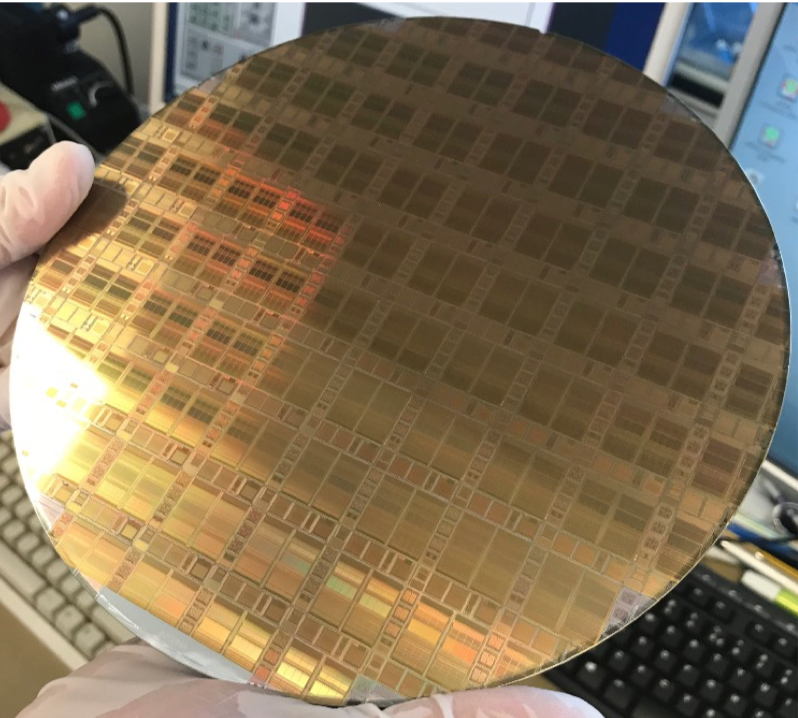
\includegraphics[width=0.49\textwidth]{figures/nsw/use_cases/verso_use_case_vmm_die}
        \raisebox{0.85cm}{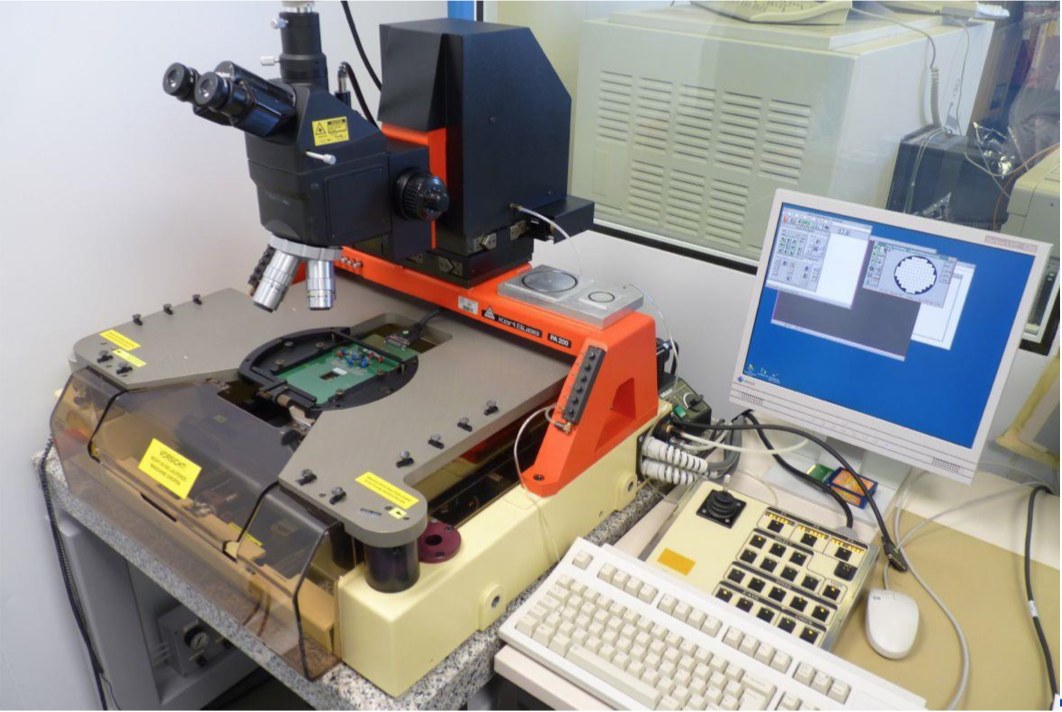
\includegraphics[width=0.49\textwidth]{figures/nsw/use_cases/verso_use_case_die_reader}}
        \caption{
            Silicon wafer testing lab at CERN.
            \textbf{\textit{Left}}: Silicon wafer die containing VMM ASIC chips prior to being cut.
                Additional ASICs are shared on the same silicon wafer, as well, so as to make efficient
                use of space on the silicon and of CHFs.
            \textbf{\textit{Right}}: The silicon wafer die is inserted into the machine on the left.
                Visual inspection of the silicon can be made via the microscope.
                The machine allows for adapter boards to be used to interface to the ASICs directly,
                via the software on the PC that controls the machine.
        }
        \label{fig:vrs_vmm_prod}
    \end{center}
\end{figure}
